%!TEX root = ../main.tex
\section{V2X for Cooperative Perception and Automated Driving}
\label{sec:cooperative_perception}

Once a reliable wireless communication link is established, vehicles can run advanced safety applications.
The most important application for high-level automated driving is Cooperative Perception (CP), also known as collective perception~\cite{etsi_cpm_2019}.
This section analyzes how V2X enables cooperative perception, examines different sensor fusion levels, defines strict quality-of-service requirements, and reviews error patterns observed in driving simulations.

\subsection{Motivation: Overcoming Sensor Blind Spots}
Autonomous vehicles depend on onboard perception sensors to observe the surrounding environment:
\begin{itemize}
    \item \textbf{Cameras:} Capture rich color, lane markings, and traffic sign semantics, but suffer under low light and direct glare.
    \item \textbf{LiDAR:} Generates accurate 3D point clouds, but degrades in heavy rain, snow, or dense fog.
    \item \textbf{Radar:} Measures object distance and velocity reliably in bad weather, but provides low angular resolution.
\end{itemize}

Despite their strengths, all onboard sensors share a major physical limitation: they require a direct line-of-sight (LOS).
In real traffic, buildings, large trucks, and road geometry frequently block this line-of-sight.
Fig.~\ref{fig:urban_cp_scenario} illustrates this problem in a typical urban intersection.
Without cooperative perception, an automated vehicle following a large delivery truck cannot see a child running across the crosswalk.
Because the front view is blocked, the vehicle cannot react in time, creating a severe collision risk.
With cooperative perception, another vehicle or an RSU on the corner detects the child and immediately transmits the pedestrian's coordinates over V2X.
The receiving vehicle processes this shared information, predicts the child's path, and brakes safely before the child enters its lane.

\begin{figure}[!t]
\centering
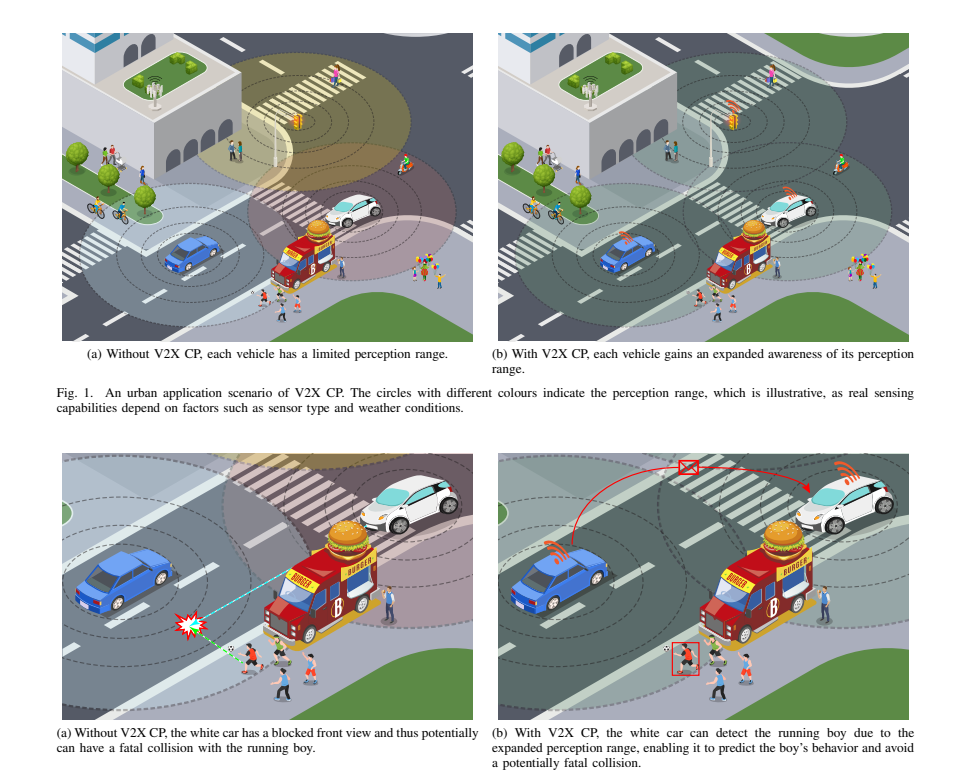
\includegraphics[width=0.98\columnwidth]{figures/rq2/rq2_urban_cooperative_perception_scenario.png}
\caption{Urban cooperative perception scenario: (a) Without V2X, the vehicle's view is blocked by a delivery truck; (b) With V2X, shared sensor data reveals the hidden pedestrian in advance.}
\label{fig:urban_cp_scenario}
\end{figure}

\subsection{Standardized Message Sets: CAM, DENM, and CPM}
To share perception data efficiently, international standardization bodies defined standard message structures:
\begin{itemize}
    \item \textbf{Cooperative Awareness Messages (CAM):} Periodic status messages broadcasted at 1 to 10~Hz.
    They include the sender's own position, speed, acceleration, and heading, but do not describe other objects.
    \item \textbf{Decentralized Environmental Notification Messages (DENM):} Event-driven messages sent when an incident occurs, such as roadworks, emergency braking, or icy roads.
    \item \textbf{Collective Perception Messages (CPM):} Standardized by ETSI in TR~103~562~\cite{etsi_cpm_2019}.
    Unlike CAMs, a CPM allows a vehicle or RSU to describe \textit{other} detected objects in its vicinity.
    A CPM contains the sender's sensor capabilities, detected obstacles (3D position, speed, dimensions, and classification confidence), and free-space perception areas.
\end{itemize}

\subsection{Sensor Fusion Strategies}
When vehicles share sensor data, they must decide at what processing stage to merge the information.
As illustrated in Fig.~\ref{fig:fusion_schemes}, cooperative perception systems use three main fusion strategies:

\begin{figure}[!t]
\centering
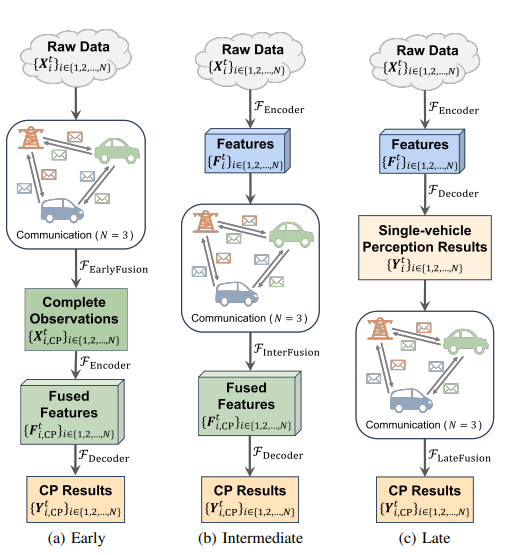
\includegraphics[width=0.95\columnwidth]{figures/rq2/rq2_fusion_schemes_early_intermediate_late.png}
\caption{The three main sensor fusion strategies in cooperative perception: (a) Early Fusion, (b) Intermediate Fusion, and (c) Late Fusion.}
\label{fig:fusion_schemes}
\end{figure}

\begin{itemize}
    \item \textbf{Early Fusion (Raw Data):} Vehicles transmit raw, unprocessed sensor measurements, such as raw camera images or full LiDAR point clouds.
    The receiver combines the raw streams before running perception models.
    \textit{Advantages:} Preserves complete geometric and semantic details, resulting in the highest detection accuracy.
    \textit{Drawbacks:} Requires massive communication bandwidth ($> 100$~Mbps per vehicle) and nanosecond-level time synchronization, which overwhelms wireless vehicular channels.
    
    \item \textbf{Late Fusion (Decision / Object Level):} Each vehicle processes its sensor data independently using its local detectors.
    Vehicles only exchange the final results: a list of detected objects with 3D bounding boxes, velocities, and confidence scores (as in ETSI CPM).
    \textit{Advantages:} Extremely low bandwidth consumption (a few kilobytes per message), making it easy to run over existing DSRC and LTE-V2X channels.
    \textit{Drawbacks:} Low accuracy under occlusion.
    If a vehicle's onboard detector fails to identify a partially visible object, that object is permanently lost because raw supporting evidence was discarded.

    \item \textbf{Intermediate Fusion (Feature Level):} Each vehicle uses a deep neural network encoder to extract compressed intermediate feature representations (latent feature maps).
    Vehicles share these feature maps over V2X, align them, and fuse them using spatial attention mechanisms or Graph Neural Networks (GNNs), such as V2X-ViT~\cite{xu2022v2xvit}, Where2comm~\cite{hu2022where2comm}, and F-Cooper~\cite{chen2019fcooper}.
    \textit{Advantages:} Represents the current state of the art by achieving detection accuracy close to early fusion while keeping bandwidth demands within realistic wireless limits.
\end{itemize}

\subsection{Coordinate Alignment and Transformation}
Before two vehicles can fuse their perception data, their coordinate systems must be aligned.
Each vehicle measures objects relative to its own local coordinate frame.
To transform a 3D point $p_B = [x_B, y_B, z_B, 1]^T$ from the sender vehicle $B$'s frame to the receiver vehicle $A$'s ego frame, the system applies the coordinate transformation in \eqref{eq:coordinate_transform}:
\begin{equation}
p_A = T_{B \to A} \cdot p_B = T_A^{-1} \cdot T_B \cdot p_B
\label{eq:coordinate_transform}
\end{equation}
where each global transformation matrix $T$ is structured as shown in \eqref{eq:matrix_t}:
\begin{equation}
T = \begin{bmatrix}
R & t \\
0 & 1
\end{bmatrix}
\label{eq:matrix_t}
\end{equation}
In \eqref{eq:matrix_t}, $t = [x, y, z]^T$ represents the $3 \times 1$ translation vector, while the rotation matrix $R = R_z(\alpha) R_y(\beta) R_x(\gamma)$ is calculated from the vehicle's yaw ($\alpha$), pitch ($\beta$), and roll ($\gamma$) angles.
If the sender vehicle has noisy GPS or IMU sensors, small angular errors create large spatial offsets when projecting objects, causing misaligned object duplicates.

\subsection{Strict Quality-of-Service (QoS) Requirements}
Cooperative perception applications demand strict communication performance:
\begin{itemize}
    \item \textbf{Ultra-Low Latency ($< 10$--$20$~ms):} When a vehicle travels at 120~km/h (33.3~m/s), a latency of 100~ms means the vehicle travels 3.3 meters before processing the shared alert.
    If transmission delay exceeds 100~ms, the spatial position of moving obstacles becomes stale, requiring extrapolation that increases tracking errors.
    If delay exceeds 500~ms, empirical studies show that cooperative perception performs worse than an isolated vehicle.
    \item \textbf{Ultra-High Reliability ($> 99.999\%$):} Missed packets during emergency maneuvers can lead directly to fatal collisions.
    Safety applications require near-perfect packet delivery within the critical braking distance.
    \item \textbf{High Update Frequency ($10$--$20$~Hz):} Fast-moving obstacles require regular position refreshes to maintain smooth trajectory tracking in Kalman filters.
\end{itemize}

\subsection{Error Taxonomy and Safety Impact in Driving Simulations}
Extensive testing in simulation environments like CARLA~\cite{dosovitskiy2017carla} and OpenCDA reveals that cooperative perception can introduce new failure modes if communication degrades.
As classified in Fig.~\ref{fig:error_taxonomy}, cooperative perception errors fall into two main categories:

\begin{figure}[!t]
\centering
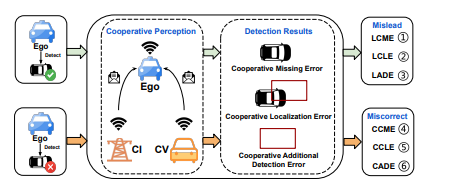
\includegraphics[width=0.92\columnwidth]{figures/rq2/rq2_cooperative_perception_error_taxonomy.png}
\caption{Taxonomy of detection errors in cooperative perception: Misleading errors (LCME, LCLE, LADE) and Miscorrecting errors (CCME, CCLE, CADE).}
\label{fig:error_taxonomy}
\end{figure}

\begin{enumerate}
    \item \textbf{Misleading Errors (LE):} Occur when the ego vehicle detected an object correctly on its own, but imperfect cooperative data corrupts the final result:
    \begin{itemize}
        \item \textit{LCME (Misleading Missing Error):} The ego vehicle saw the object, but shared data causes the object to disappear from the fused map.
        \item \textit{LCLE (Misleading Localization Error):} The ego vehicle localized the object accurately, but cooperative fusion shifts the bounding box into the wrong position.
        \item \textit{LADE (Misleading Additional Detection Error):} Cooperative fusion introduces a ghost obstacle that does not exist in reality, triggering phantom braking.
    \end{itemize}
    \item \textbf{Miscorrecting Errors (CE):} Occur when the ego vehicle failed to detect an obstacle, and the cooperative network fails to fix or worsens the mistake:
    \begin{itemize}
        \item \textit{CCME (Miscorrected Missing Error):} Both the ego vehicle and cooperative partners fail to detect the obstacle.
        \item \textit{CCLE (Miscorrected Localization Error):} Both nodes detect the object with large spatial errors.
        \item \textit{CADE (Miscorrected Additional Detection Error):} The cooperative network confirms a false-positive ghost detection.
    \end{itemize}
\end{enumerate}

Simulation trials demonstrate that communication latency primarily triggers LCLE and CCME errors.
For example, if an approaching perpendicular car is reported with a delay at an intersection, the ego vehicle assumes the road is clear, enters the junction, and collides.
These failure patterns show that cooperative perception cannot rely on wireless data blindly; vehicles must verify message freshness and data consistency before acting.
